%%%%%%%%%%%%%%%%%%%%%%%%%%%%%%%%%%%%%%%%%%%%%%%%%%%%%%%%%%%%%%%%%%%%%%%%%%%%%%%%%
%
% Jasi's part <3
%
%%%%%%%%%%%%%%%%%%%%%%%%%%%%%%%%%%%%%%%%%%%%%%%%%%%%%%%%%%%%%%%%%%%%%%%%%%%%%%%%%
\section{UltraStereoAlgorithm}
\subsection{}

\begin{frame}{UltraStereo}
\begin{itemize}
\item 2 IR cameras: monochrome Ximea cameras, 1280x1024 pixel at 210Hz
\item DOE projector
\end{itemize}
\end{frame}

\begin{frame}

\begin{figure}
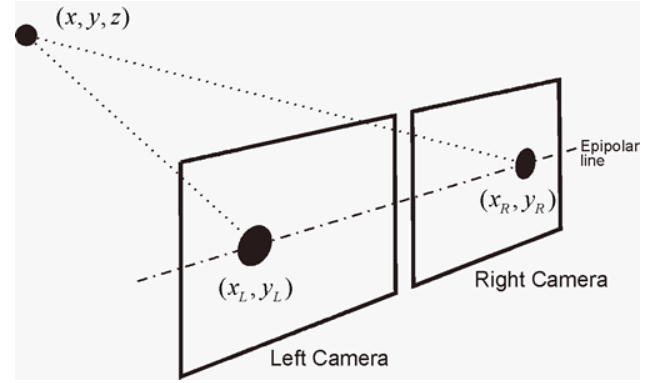
\includegraphics[scale=0.5]{pictures/disp}
\end{figure}
\begin{equation}
disparity = \frac{bf}{x_{L}- x_{R}}
\end{equation}
f = focal length\\
b = baseline
\end{frame}

\begin{frame}{Dimensionality Reduction}
\begin{figure}
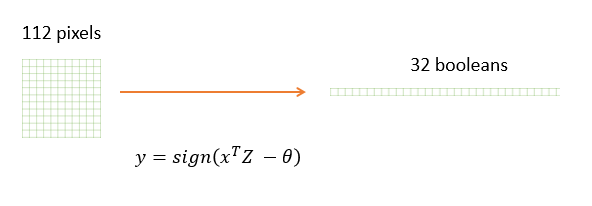
\includegraphics[scale=0.6]{pictures/patches}
\end{figure}
$ x \in R^{W} $  with W = 11x11\\
$ Z \in R^{b} $ with b = 32\\
$ \theta \in R^b$
$ y \in (0,1)^{b}$
\end{frame}

\begin {frame}{How to chose the parameters}
\begin {figure}
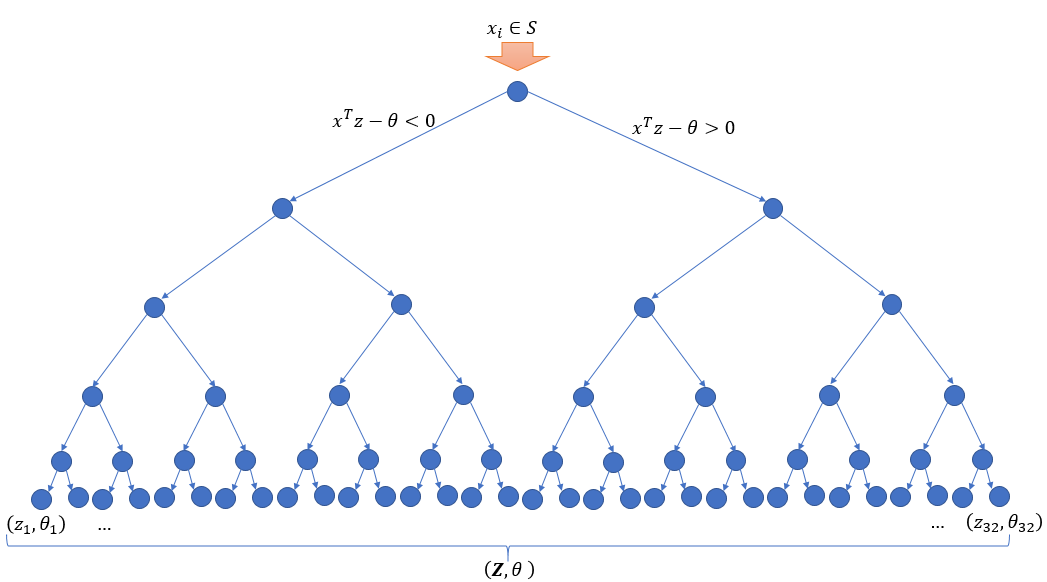
\includegraphics[scale=0.35]{pictures/tree}
\end {figure}

\begin{itemize}
\item k<< W -> sparse hyperplanes
\item Information gain: $I(\delta) = H(S) -\sum_{d\in L,R} \frac{S_{d}(\delta)}{S} H(S_{d}(\delta))$
\end{itemize}
$\delta$: set of learned parameters $(z,\theta)$
\end{frame}
